The main goal of our project was to correctly identify handwritten digits based on the MNIST  ("Modified National Institute of Standards and Technology") data set.
This data set consists of 42,000 gray-scale images. Each image is 28 pixels in height and 28 pixels in width. Each pixel has a single pixel-value associated with it, indicating the lightness or darkness of that pixel \cite{kaggel}.

\begin{figure}[h]
	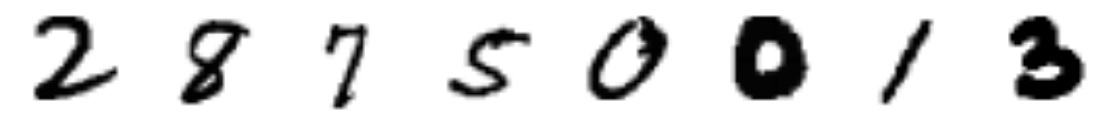
\includegraphics[width=1\textwidth, center]{Digits2}
	\caption{Visualization of eight of these images}
\end{figure}


Formally speaking, we have points  $\{x_i\}_{i=1}^l \subset \R^{28^2}$ with respective labels from $\{0,1,\ldots, 9\}$. Our goal is to now find a classification function $f$ that gives for each of these points a prediction $f(x) \in \{0,1,\ldots, 9\}$ which ideally matches the actual label.\\

There are several ways to achieve this goal, one of which is the concept of {kernelized} support vector machines (SVM). The main idea behind this algorithm is to not only separate the data according to their labels, but also to do so in a way that is as reasonable as possible, i.e. we want to maximize the distance of the data to the decision boundary. We first transfer the data with a feature map $\Phi$ into a suitable feature space and look for a linear separation there.\\

From this notion, two particular problems arise. Firstly how to solve the optimization problem of maximizing the margin (cf. Section 1.1 and 2) and secondly: The SVM is a binary classifier, i.e. it can only handle data that is divided into two classes. We therefore decided to compare different ways to deal with this obstacle, generalizing the application of SVMs to multiclass  classification problems (cf. Section \ref{ch_multiclass}). The methods that we considered all combine several instances of the SVM in its original form, classifying according to labels $\{\pm 1\}$.\\

We can summarize this binary classification problem in the objective of finding a decision function of the form
\begin{equation*}
f(x) = \sign \left(w^T\Phi(x) + b\right).
\end{equation*}


\subsection{Binary Support Vector Machine}


Approaching binary support vector machines from a more technical side, we find that they aim to find the maximum margin hyperplane in the feature space, i.e. the goal is to maximize the margin while softly penalizing points that lie on the wrong side of the boundary or inside the margin \cite{Bishop2006}. Dualizing this optimization problem, we obtain the following equivalent quadratic program:

\begin{eqnarray}
	\text{minimize} & d(\alpha) := \frac{1}{2} \alpha^T Q \alpha - 1^T \alpha \label{eq:dual_problem} \\ 
	\text{s.t.} &  0 \leq \alpha \leq C  \quad \text{and} \quad 	y^T \alpha = 0,	\nonumber
\end{eqnarray}

where $\alpha$ is the dual variable, $Q_{ij} = y_i y_j k(x_i,x_j)$, $k$ the kernel function and $C = 1/(2 \lambda l)$ for the penalty term $\lambda$ of the soft margin SVM.
After finding the optimal solution $\alpha^*$ of this program, we can formulate the resulting decision function as
\begin{equation*}
f(x) = \operatorname{sgn}\left(\sum_{i=1}^{l}\alpha^*_i y_i k(x_i,x_j)+b\right).
\end{equation*}
Note that only data points $x_i$ with $\alpha_i \neq 0$ appear in the decision function. Those points are called \textit{support vectors}.\\
By analyzing primal, dual and the corresponding KKT conditions, we find that any $x_i$ with $\alpha_i = C$ was correctly classified and lies exactly on the margin boundary, and any $x_i$ with $0<\alpha_i < C$ lies either inside the margin or on the wrong side of the margin. Additionally, any data points $x_i$ on the (correct) margin boundary must satisfy $y_i f(x_i) = 1$. We can use this property to find the parameter $b$ \cite{Bishop2006}. Hence, if we succeed to find an optimal solution to \eqref{eq:dual_problem}, we have everything we need to construct the decision function.

